
% Default to the notebook output style

    


% Inherit from the specified cell style.




    
\documentclass[11pt]{article}

    
    
    \usepackage[T1]{fontenc}
    % Nicer default font (+ math font) than Computer Modern for most use cases
    \usepackage{mathpazo}

    % Basic figure setup, for now with no caption control since it's done
    % automatically by Pandoc (which extracts ![](path) syntax from Markdown).
    \usepackage{graphicx}
    % We will generate all images so they have a width \maxwidth. This means
    % that they will get their normal width if they fit onto the page, but
    % are scaled down if they would overflow the margins.
    \makeatletter
    \def\maxwidth{\ifdim\Gin@nat@width>\linewidth\linewidth
    \else\Gin@nat@width\fi}
    \makeatother
    \let\Oldincludegraphics\includegraphics
    % Set max figure width to be 80% of text width, for now hardcoded.
    \renewcommand{\includegraphics}[1]{\Oldincludegraphics[width=.8\maxwidth]{#1}}
    % Ensure that by default, figures have no caption (until we provide a
    % proper Figure object with a Caption API and a way to capture that
    % in the conversion process - todo).
    \usepackage{caption}
    \DeclareCaptionLabelFormat{nolabel}{}
    \captionsetup{labelformat=nolabel}

    \usepackage{adjustbox} % Used to constrain images to a maximum size 
    \usepackage{xcolor} % Allow colors to be defined
    \usepackage{enumerate} % Needed for markdown enumerations to work
    \usepackage{geometry} % Used to adjust the document margins
    \usepackage{amsmath} % Equations
    \usepackage{amssymb} % Equations
    \usepackage{textcomp} % defines textquotesingle
    % Hack from http://tex.stackexchange.com/a/47451/13684:
    \AtBeginDocument{%
        \def\PYZsq{\textquotesingle}% Upright quotes in Pygmentized code
    }
    \usepackage{upquote} % Upright quotes for verbatim code
    \usepackage{eurosym} % defines \euro
    \usepackage[mathletters]{ucs} % Extended unicode (utf-8) support
    \usepackage[utf8x]{inputenc} % Allow utf-8 characters in the tex document
    \usepackage{fancyvrb} % verbatim replacement that allows latex
    \usepackage{grffile} % extends the file name processing of package graphics 
                         % to support a larger range 
    % The hyperref package gives us a pdf with properly built
    % internal navigation ('pdf bookmarks' for the table of contents,
    % internal cross-reference links, web links for URLs, etc.)
    \usepackage{hyperref}
    \usepackage{longtable} % longtable support required by pandoc >1.10
    \usepackage{booktabs}  % table support for pandoc > 1.12.2
    \usepackage[inline]{enumitem} % IRkernel/repr support (it uses the enumerate* environment)
    \usepackage[normalem]{ulem} % ulem is needed to support strikethroughs (\sout)
                                % normalem makes italics be italics, not underlines
    

    
    
    % Colors for the hyperref package
    \definecolor{urlcolor}{rgb}{0,.145,.698}
    \definecolor{linkcolor}{rgb}{.71,0.21,0.01}
    \definecolor{citecolor}{rgb}{.12,.54,.11}

    % ANSI colors
    \definecolor{ansi-black}{HTML}{3E424D}
    \definecolor{ansi-black-intense}{HTML}{282C36}
    \definecolor{ansi-red}{HTML}{E75C58}
    \definecolor{ansi-red-intense}{HTML}{B22B31}
    \definecolor{ansi-green}{HTML}{00A250}
    \definecolor{ansi-green-intense}{HTML}{007427}
    \definecolor{ansi-yellow}{HTML}{DDB62B}
    \definecolor{ansi-yellow-intense}{HTML}{B27D12}
    \definecolor{ansi-blue}{HTML}{208FFB}
    \definecolor{ansi-blue-intense}{HTML}{0065CA}
    \definecolor{ansi-magenta}{HTML}{D160C4}
    \definecolor{ansi-magenta-intense}{HTML}{A03196}
    \definecolor{ansi-cyan}{HTML}{60C6C8}
    \definecolor{ansi-cyan-intense}{HTML}{258F8F}
    \definecolor{ansi-white}{HTML}{C5C1B4}
    \definecolor{ansi-white-intense}{HTML}{A1A6B2}

    % commands and environments needed by pandoc snippets
    % extracted from the output of `pandoc -s`
    \providecommand{\tightlist}{%
      \setlength{\itemsep}{0pt}\setlength{\parskip}{0pt}}
    \DefineVerbatimEnvironment{Highlighting}{Verbatim}{commandchars=\\\{\}}
    % Add ',fontsize=\small' for more characters per line
    \newenvironment{Shaded}{}{}
    \newcommand{\KeywordTok}[1]{\textcolor[rgb]{0.00,0.44,0.13}{\textbf{{#1}}}}
    \newcommand{\DataTypeTok}[1]{\textcolor[rgb]{0.56,0.13,0.00}{{#1}}}
    \newcommand{\DecValTok}[1]{\textcolor[rgb]{0.25,0.63,0.44}{{#1}}}
    \newcommand{\BaseNTok}[1]{\textcolor[rgb]{0.25,0.63,0.44}{{#1}}}
    \newcommand{\FloatTok}[1]{\textcolor[rgb]{0.25,0.63,0.44}{{#1}}}
    \newcommand{\CharTok}[1]{\textcolor[rgb]{0.25,0.44,0.63}{{#1}}}
    \newcommand{\StringTok}[1]{\textcolor[rgb]{0.25,0.44,0.63}{{#1}}}
    \newcommand{\CommentTok}[1]{\textcolor[rgb]{0.38,0.63,0.69}{\textit{{#1}}}}
    \newcommand{\OtherTok}[1]{\textcolor[rgb]{0.00,0.44,0.13}{{#1}}}
    \newcommand{\AlertTok}[1]{\textcolor[rgb]{1.00,0.00,0.00}{\textbf{{#1}}}}
    \newcommand{\FunctionTok}[1]{\textcolor[rgb]{0.02,0.16,0.49}{{#1}}}
    \newcommand{\RegionMarkerTok}[1]{{#1}}
    \newcommand{\ErrorTok}[1]{\textcolor[rgb]{1.00,0.00,0.00}{\textbf{{#1}}}}
    \newcommand{\NormalTok}[1]{{#1}}
    
    % Additional commands for more recent versions of Pandoc
    \newcommand{\ConstantTok}[1]{\textcolor[rgb]{0.53,0.00,0.00}{{#1}}}
    \newcommand{\SpecialCharTok}[1]{\textcolor[rgb]{0.25,0.44,0.63}{{#1}}}
    \newcommand{\VerbatimStringTok}[1]{\textcolor[rgb]{0.25,0.44,0.63}{{#1}}}
    \newcommand{\SpecialStringTok}[1]{\textcolor[rgb]{0.73,0.40,0.53}{{#1}}}
    \newcommand{\ImportTok}[1]{{#1}}
    \newcommand{\DocumentationTok}[1]{\textcolor[rgb]{0.73,0.13,0.13}{\textit{{#1}}}}
    \newcommand{\AnnotationTok}[1]{\textcolor[rgb]{0.38,0.63,0.69}{\textbf{\textit{{#1}}}}}
    \newcommand{\CommentVarTok}[1]{\textcolor[rgb]{0.38,0.63,0.69}{\textbf{\textit{{#1}}}}}
    \newcommand{\VariableTok}[1]{\textcolor[rgb]{0.10,0.09,0.49}{{#1}}}
    \newcommand{\ControlFlowTok}[1]{\textcolor[rgb]{0.00,0.44,0.13}{\textbf{{#1}}}}
    \newcommand{\OperatorTok}[1]{\textcolor[rgb]{0.40,0.40,0.40}{{#1}}}
    \newcommand{\BuiltInTok}[1]{{#1}}
    \newcommand{\ExtensionTok}[1]{{#1}}
    \newcommand{\PreprocessorTok}[1]{\textcolor[rgb]{0.74,0.48,0.00}{{#1}}}
    \newcommand{\AttributeTok}[1]{\textcolor[rgb]{0.49,0.56,0.16}{{#1}}}
    \newcommand{\InformationTok}[1]{\textcolor[rgb]{0.38,0.63,0.69}{\textbf{\textit{{#1}}}}}
    \newcommand{\WarningTok}[1]{\textcolor[rgb]{0.38,0.63,0.69}{\textbf{\textit{{#1}}}}}
    
    
    % Define a nice break command that doesn't care if a line doesn't already
    % exist.
    \def\br{\hspace*{\fill} \\* }
    % Math Jax compatability definitions
    \def\gt{>}
    \def\lt{<}
    % Document parameters
    \title{Tutorial-1.1-Weighted\_predictions\_matrix\_approach}
    
    
    

    % Pygments definitions
    
\makeatletter
\def\PY@reset{\let\PY@it=\relax \let\PY@bf=\relax%
    \let\PY@ul=\relax \let\PY@tc=\relax%
    \let\PY@bc=\relax \let\PY@ff=\relax}
\def\PY@tok#1{\csname PY@tok@#1\endcsname}
\def\PY@toks#1+{\ifx\relax#1\empty\else%
    \PY@tok{#1}\expandafter\PY@toks\fi}
\def\PY@do#1{\PY@bc{\PY@tc{\PY@ul{%
    \PY@it{\PY@bf{\PY@ff{#1}}}}}}}
\def\PY#1#2{\PY@reset\PY@toks#1+\relax+\PY@do{#2}}

\expandafter\def\csname PY@tok@w\endcsname{\def\PY@tc##1{\textcolor[rgb]{0.73,0.73,0.73}{##1}}}
\expandafter\def\csname PY@tok@c\endcsname{\let\PY@it=\textit\def\PY@tc##1{\textcolor[rgb]{0.25,0.50,0.50}{##1}}}
\expandafter\def\csname PY@tok@cp\endcsname{\def\PY@tc##1{\textcolor[rgb]{0.74,0.48,0.00}{##1}}}
\expandafter\def\csname PY@tok@k\endcsname{\let\PY@bf=\textbf\def\PY@tc##1{\textcolor[rgb]{0.00,0.50,0.00}{##1}}}
\expandafter\def\csname PY@tok@kp\endcsname{\def\PY@tc##1{\textcolor[rgb]{0.00,0.50,0.00}{##1}}}
\expandafter\def\csname PY@tok@kt\endcsname{\def\PY@tc##1{\textcolor[rgb]{0.69,0.00,0.25}{##1}}}
\expandafter\def\csname PY@tok@o\endcsname{\def\PY@tc##1{\textcolor[rgb]{0.40,0.40,0.40}{##1}}}
\expandafter\def\csname PY@tok@ow\endcsname{\let\PY@bf=\textbf\def\PY@tc##1{\textcolor[rgb]{0.67,0.13,1.00}{##1}}}
\expandafter\def\csname PY@tok@nb\endcsname{\def\PY@tc##1{\textcolor[rgb]{0.00,0.50,0.00}{##1}}}
\expandafter\def\csname PY@tok@nf\endcsname{\def\PY@tc##1{\textcolor[rgb]{0.00,0.00,1.00}{##1}}}
\expandafter\def\csname PY@tok@nc\endcsname{\let\PY@bf=\textbf\def\PY@tc##1{\textcolor[rgb]{0.00,0.00,1.00}{##1}}}
\expandafter\def\csname PY@tok@nn\endcsname{\let\PY@bf=\textbf\def\PY@tc##1{\textcolor[rgb]{0.00,0.00,1.00}{##1}}}
\expandafter\def\csname PY@tok@ne\endcsname{\let\PY@bf=\textbf\def\PY@tc##1{\textcolor[rgb]{0.82,0.25,0.23}{##1}}}
\expandafter\def\csname PY@tok@nv\endcsname{\def\PY@tc##1{\textcolor[rgb]{0.10,0.09,0.49}{##1}}}
\expandafter\def\csname PY@tok@no\endcsname{\def\PY@tc##1{\textcolor[rgb]{0.53,0.00,0.00}{##1}}}
\expandafter\def\csname PY@tok@nl\endcsname{\def\PY@tc##1{\textcolor[rgb]{0.63,0.63,0.00}{##1}}}
\expandafter\def\csname PY@tok@ni\endcsname{\let\PY@bf=\textbf\def\PY@tc##1{\textcolor[rgb]{0.60,0.60,0.60}{##1}}}
\expandafter\def\csname PY@tok@na\endcsname{\def\PY@tc##1{\textcolor[rgb]{0.49,0.56,0.16}{##1}}}
\expandafter\def\csname PY@tok@nt\endcsname{\let\PY@bf=\textbf\def\PY@tc##1{\textcolor[rgb]{0.00,0.50,0.00}{##1}}}
\expandafter\def\csname PY@tok@nd\endcsname{\def\PY@tc##1{\textcolor[rgb]{0.67,0.13,1.00}{##1}}}
\expandafter\def\csname PY@tok@s\endcsname{\def\PY@tc##1{\textcolor[rgb]{0.73,0.13,0.13}{##1}}}
\expandafter\def\csname PY@tok@sd\endcsname{\let\PY@it=\textit\def\PY@tc##1{\textcolor[rgb]{0.73,0.13,0.13}{##1}}}
\expandafter\def\csname PY@tok@si\endcsname{\let\PY@bf=\textbf\def\PY@tc##1{\textcolor[rgb]{0.73,0.40,0.53}{##1}}}
\expandafter\def\csname PY@tok@se\endcsname{\let\PY@bf=\textbf\def\PY@tc##1{\textcolor[rgb]{0.73,0.40,0.13}{##1}}}
\expandafter\def\csname PY@tok@sr\endcsname{\def\PY@tc##1{\textcolor[rgb]{0.73,0.40,0.53}{##1}}}
\expandafter\def\csname PY@tok@ss\endcsname{\def\PY@tc##1{\textcolor[rgb]{0.10,0.09,0.49}{##1}}}
\expandafter\def\csname PY@tok@sx\endcsname{\def\PY@tc##1{\textcolor[rgb]{0.00,0.50,0.00}{##1}}}
\expandafter\def\csname PY@tok@m\endcsname{\def\PY@tc##1{\textcolor[rgb]{0.40,0.40,0.40}{##1}}}
\expandafter\def\csname PY@tok@gh\endcsname{\let\PY@bf=\textbf\def\PY@tc##1{\textcolor[rgb]{0.00,0.00,0.50}{##1}}}
\expandafter\def\csname PY@tok@gu\endcsname{\let\PY@bf=\textbf\def\PY@tc##1{\textcolor[rgb]{0.50,0.00,0.50}{##1}}}
\expandafter\def\csname PY@tok@gd\endcsname{\def\PY@tc##1{\textcolor[rgb]{0.63,0.00,0.00}{##1}}}
\expandafter\def\csname PY@tok@gi\endcsname{\def\PY@tc##1{\textcolor[rgb]{0.00,0.63,0.00}{##1}}}
\expandafter\def\csname PY@tok@gr\endcsname{\def\PY@tc##1{\textcolor[rgb]{1.00,0.00,0.00}{##1}}}
\expandafter\def\csname PY@tok@ge\endcsname{\let\PY@it=\textit}
\expandafter\def\csname PY@tok@gs\endcsname{\let\PY@bf=\textbf}
\expandafter\def\csname PY@tok@gp\endcsname{\let\PY@bf=\textbf\def\PY@tc##1{\textcolor[rgb]{0.00,0.00,0.50}{##1}}}
\expandafter\def\csname PY@tok@go\endcsname{\def\PY@tc##1{\textcolor[rgb]{0.53,0.53,0.53}{##1}}}
\expandafter\def\csname PY@tok@gt\endcsname{\def\PY@tc##1{\textcolor[rgb]{0.00,0.27,0.87}{##1}}}
\expandafter\def\csname PY@tok@err\endcsname{\def\PY@bc##1{\setlength{\fboxsep}{0pt}\fcolorbox[rgb]{1.00,0.00,0.00}{1,1,1}{\strut ##1}}}
\expandafter\def\csname PY@tok@kc\endcsname{\let\PY@bf=\textbf\def\PY@tc##1{\textcolor[rgb]{0.00,0.50,0.00}{##1}}}
\expandafter\def\csname PY@tok@kd\endcsname{\let\PY@bf=\textbf\def\PY@tc##1{\textcolor[rgb]{0.00,0.50,0.00}{##1}}}
\expandafter\def\csname PY@tok@kn\endcsname{\let\PY@bf=\textbf\def\PY@tc##1{\textcolor[rgb]{0.00,0.50,0.00}{##1}}}
\expandafter\def\csname PY@tok@kr\endcsname{\let\PY@bf=\textbf\def\PY@tc##1{\textcolor[rgb]{0.00,0.50,0.00}{##1}}}
\expandafter\def\csname PY@tok@bp\endcsname{\def\PY@tc##1{\textcolor[rgb]{0.00,0.50,0.00}{##1}}}
\expandafter\def\csname PY@tok@fm\endcsname{\def\PY@tc##1{\textcolor[rgb]{0.00,0.00,1.00}{##1}}}
\expandafter\def\csname PY@tok@vc\endcsname{\def\PY@tc##1{\textcolor[rgb]{0.10,0.09,0.49}{##1}}}
\expandafter\def\csname PY@tok@vg\endcsname{\def\PY@tc##1{\textcolor[rgb]{0.10,0.09,0.49}{##1}}}
\expandafter\def\csname PY@tok@vi\endcsname{\def\PY@tc##1{\textcolor[rgb]{0.10,0.09,0.49}{##1}}}
\expandafter\def\csname PY@tok@vm\endcsname{\def\PY@tc##1{\textcolor[rgb]{0.10,0.09,0.49}{##1}}}
\expandafter\def\csname PY@tok@sa\endcsname{\def\PY@tc##1{\textcolor[rgb]{0.73,0.13,0.13}{##1}}}
\expandafter\def\csname PY@tok@sb\endcsname{\def\PY@tc##1{\textcolor[rgb]{0.73,0.13,0.13}{##1}}}
\expandafter\def\csname PY@tok@sc\endcsname{\def\PY@tc##1{\textcolor[rgb]{0.73,0.13,0.13}{##1}}}
\expandafter\def\csname PY@tok@dl\endcsname{\def\PY@tc##1{\textcolor[rgb]{0.73,0.13,0.13}{##1}}}
\expandafter\def\csname PY@tok@s2\endcsname{\def\PY@tc##1{\textcolor[rgb]{0.73,0.13,0.13}{##1}}}
\expandafter\def\csname PY@tok@sh\endcsname{\def\PY@tc##1{\textcolor[rgb]{0.73,0.13,0.13}{##1}}}
\expandafter\def\csname PY@tok@s1\endcsname{\def\PY@tc##1{\textcolor[rgb]{0.73,0.13,0.13}{##1}}}
\expandafter\def\csname PY@tok@mb\endcsname{\def\PY@tc##1{\textcolor[rgb]{0.40,0.40,0.40}{##1}}}
\expandafter\def\csname PY@tok@mf\endcsname{\def\PY@tc##1{\textcolor[rgb]{0.40,0.40,0.40}{##1}}}
\expandafter\def\csname PY@tok@mh\endcsname{\def\PY@tc##1{\textcolor[rgb]{0.40,0.40,0.40}{##1}}}
\expandafter\def\csname PY@tok@mi\endcsname{\def\PY@tc##1{\textcolor[rgb]{0.40,0.40,0.40}{##1}}}
\expandafter\def\csname PY@tok@il\endcsname{\def\PY@tc##1{\textcolor[rgb]{0.40,0.40,0.40}{##1}}}
\expandafter\def\csname PY@tok@mo\endcsname{\def\PY@tc##1{\textcolor[rgb]{0.40,0.40,0.40}{##1}}}
\expandafter\def\csname PY@tok@ch\endcsname{\let\PY@it=\textit\def\PY@tc##1{\textcolor[rgb]{0.25,0.50,0.50}{##1}}}
\expandafter\def\csname PY@tok@cm\endcsname{\let\PY@it=\textit\def\PY@tc##1{\textcolor[rgb]{0.25,0.50,0.50}{##1}}}
\expandafter\def\csname PY@tok@cpf\endcsname{\let\PY@it=\textit\def\PY@tc##1{\textcolor[rgb]{0.25,0.50,0.50}{##1}}}
\expandafter\def\csname PY@tok@c1\endcsname{\let\PY@it=\textit\def\PY@tc##1{\textcolor[rgb]{0.25,0.50,0.50}{##1}}}
\expandafter\def\csname PY@tok@cs\endcsname{\let\PY@it=\textit\def\PY@tc##1{\textcolor[rgb]{0.25,0.50,0.50}{##1}}}

\def\PYZbs{\char`\\}
\def\PYZus{\char`\_}
\def\PYZob{\char`\{}
\def\PYZcb{\char`\}}
\def\PYZca{\char`\^}
\def\PYZam{\char`\&}
\def\PYZlt{\char`\<}
\def\PYZgt{\char`\>}
\def\PYZsh{\char`\#}
\def\PYZpc{\char`\%}
\def\PYZdl{\char`\$}
\def\PYZhy{\char`\-}
\def\PYZsq{\char`\'}
\def\PYZdq{\char`\"}
\def\PYZti{\char`\~}
% for compatibility with earlier versions
\def\PYZat{@}
\def\PYZlb{[}
\def\PYZrb{]}
\makeatother


    % Exact colors from NB
    \definecolor{incolor}{rgb}{0.0, 0.0, 0.5}
    \definecolor{outcolor}{rgb}{0.545, 0.0, 0.0}



    
    % Prevent overflowing lines due to hard-to-break entities
    \sloppy 
    % Setup hyperref package
    \hypersetup{
      breaklinks=true,  % so long urls are correctly broken across lines
      colorlinks=true,
      urlcolor=urlcolor,
      linkcolor=linkcolor,
      citecolor=citecolor,
      }
    % Slightly bigger margins than the latex defaults
    
    \geometry{verbose,tmargin=1in,bmargin=1in,lmargin=1in,rmargin=1in}
    
    

    \begin{document}
    
    
    \maketitle
    
    

    
    \section{Weighted-predictions matrix}\label{weighted-predictions-matrix}

The weighted-predictions matrix, \(W\), introduced by
\href{https://doi.org/10.1890/0012-9658\%282002\%29083\%5B1372:ROCSIA\%5D2.0.CO;2}{Dambacher
et al. (2002)}, summarises the positive and negative effects of a
press-perturbation on species in an interaction network. In this
tutorial, we obtain \(W\) for the example from the paper, and use it to
predict the effects of a negative press-perturbation of species 3 on
species 3, 4, and 5 in the network below.

    \begin{Verbatim}[commandchars=\\\{\}]
{\color{incolor}In [{\color{incolor}20}]:} \PY{k+kn}{from} \PY{n+nn}{IPython.display} \PY{k+kn}{import} \PY{n}{IFrame}
         \PY{k+kn}{from} \PY{n+nn}{IPython.display} \PY{k+kn}{import} \PY{n}{Image}
         \PY{k+kn}{import} \PY{n+nn}{os}
         
         \PY{c+c1}{\PYZsh{} display the interaction network used in the example}
         \PY{c+c1}{\PYZsh{}IFrame(\PYZdq{}fivevariable2.pdf\PYZdq{}, width=500, height=400)}
\end{Verbatim}


    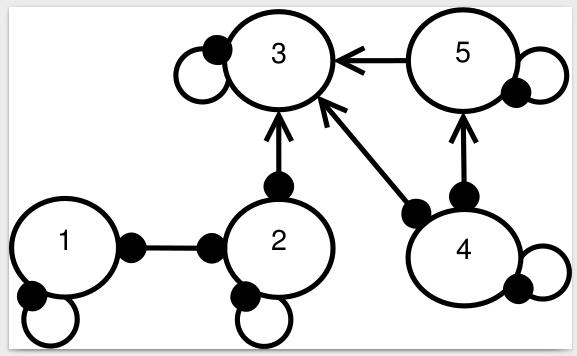
\includegraphics{fivevariable2.png} \texttt{fivevariable2.png}

    \subsection{Obtain the weighted-predictions
matrix}\label{obtain-the-weighted-predictions-matrix}

\subsubsection{Step 1: Create the qualitative community
matrix}\label{step-1-create-the-qualitative-community-matrix}

It is convenient to start by encoding the interaction network in a
flexible way. Below we have a list of species, \texttt{spp\_list}, a
dictionary that specifies the positive interactions between species,
\texttt{positive\_edges\_dict}, and a dictionary that specifies the
negative interactions between species, \texttt{negative\_edges\_dict}.

    \begin{Verbatim}[commandchars=\\\{\}]
{\color{incolor}In [{\color{incolor}21}]:} \PY{c+c1}{\PYZsh{}}
         \PY{n}{spp\PYZus{}list} \PY{o}{=} \PY{p}{[}\PY{l+s+s1}{\PYZsq{}}\PY{l+s+s1}{s1}\PY{l+s+s1}{\PYZsq{}}\PY{p}{,}\PY{l+s+s1}{\PYZsq{}}\PY{l+s+s1}{s2}\PY{l+s+s1}{\PYZsq{}}\PY{p}{,}\PY{l+s+s1}{\PYZsq{}}\PY{l+s+s1}{s3}\PY{l+s+s1}{\PYZsq{}}\PY{p}{,}\PY{l+s+s1}{\PYZsq{}}\PY{l+s+s1}{s4}\PY{l+s+s1}{\PYZsq{}}\PY{p}{,}\PY{l+s+s1}{\PYZsq{}}\PY{l+s+s1}{s5}\PY{l+s+s1}{\PYZsq{}}\PY{p}{]}
         
         \PY{c+c1}{\PYZsh{} key is recipient of a positive effect}
         \PY{n}{positive\PYZus{}edges\PYZus{}dict} \PY{o}{=} \PY{p}{\PYZob{}}
         \PY{l+s+s1}{\PYZsq{}}\PY{l+s+s1}{s5}\PY{l+s+s1}{\PYZsq{}}\PY{p}{:} \PY{p}{[}\PY{l+s+s1}{\PYZsq{}}\PY{l+s+s1}{s4}\PY{l+s+s1}{\PYZsq{}}\PY{p}{]}\PY{p}{,}
         \PY{l+s+s1}{\PYZsq{}}\PY{l+s+s1}{s3}\PY{l+s+s1}{\PYZsq{}}\PY{p}{:} \PY{p}{[}\PY{l+s+s1}{\PYZsq{}}\PY{l+s+s1}{s2}\PY{l+s+s1}{\PYZsq{}}\PY{p}{,} \PY{l+s+s1}{\PYZsq{}}\PY{l+s+s1}{s4}\PY{l+s+s1}{\PYZsq{}}\PY{p}{,} \PY{l+s+s1}{\PYZsq{}}\PY{l+s+s1}{s5}\PY{l+s+s1}{\PYZsq{}}\PY{p}{]}\PY{p}{,}
         \PY{p}{\PYZcb{}}
         
         \PY{c+c1}{\PYZsh{} key is recipient of a negative effect}
         \PY{n}{negative\PYZus{}edges\PYZus{}dict} \PY{o}{=} \PY{p}{\PYZob{}}
         \PY{l+s+s1}{\PYZsq{}}\PY{l+s+s1}{s5}\PY{l+s+s1}{\PYZsq{}}\PY{p}{:} \PY{p}{[}\PY{l+s+s1}{\PYZsq{}}\PY{l+s+s1}{s5}\PY{l+s+s1}{\PYZsq{}}\PY{p}{]}\PY{p}{,}
         \PY{l+s+s1}{\PYZsq{}}\PY{l+s+s1}{s4}\PY{l+s+s1}{\PYZsq{}}\PY{p}{:} \PY{p}{[}\PY{l+s+s1}{\PYZsq{}}\PY{l+s+s1}{s4}\PY{l+s+s1}{\PYZsq{}}\PY{p}{,} \PY{l+s+s1}{\PYZsq{}}\PY{l+s+s1}{s5}\PY{l+s+s1}{\PYZsq{}}\PY{p}{,} \PY{l+s+s1}{\PYZsq{}}\PY{l+s+s1}{s3}\PY{l+s+s1}{\PYZsq{}}\PY{p}{]}\PY{p}{,}
         \PY{l+s+s1}{\PYZsq{}}\PY{l+s+s1}{s3}\PY{l+s+s1}{\PYZsq{}}\PY{p}{:} \PY{p}{[}\PY{l+s+s1}{\PYZsq{}}\PY{l+s+s1}{s3}\PY{l+s+s1}{\PYZsq{}}\PY{p}{]}\PY{p}{,}
         \PY{l+s+s1}{\PYZsq{}}\PY{l+s+s1}{s2}\PY{l+s+s1}{\PYZsq{}}\PY{p}{:} \PY{p}{[}\PY{l+s+s1}{\PYZsq{}}\PY{l+s+s1}{s2}\PY{l+s+s1}{\PYZsq{}}\PY{p}{,} \PY{l+s+s1}{\PYZsq{}}\PY{l+s+s1}{s1}\PY{l+s+s1}{\PYZsq{}}\PY{p}{,} \PY{l+s+s1}{\PYZsq{}}\PY{l+s+s1}{s3}\PY{l+s+s1}{\PYZsq{}}\PY{p}{]}\PY{p}{,}
         \PY{l+s+s1}{\PYZsq{}}\PY{l+s+s1}{s1}\PY{l+s+s1}{\PYZsq{}}\PY{p}{:} \PY{p}{[}\PY{l+s+s1}{\PYZsq{}}\PY{l+s+s1}{s1}\PY{l+s+s1}{\PYZsq{}}\PY{p}{,} \PY{l+s+s1}{\PYZsq{}}\PY{l+s+s1}{s2}\PY{l+s+s1}{\PYZsq{}}\PY{p}{]}\PY{p}{,}
         \PY{p}{\PYZcb{}}
\end{Verbatim}


    The qualitative community matrix, denoted \(^\circ A\) in Dambacher et
al. (2002), has a \texttt{-1} for negative species interactions,
\texttt{+1} for positive interactions, and \texttt{0} otherwise.

The first step is to assign each species name to an index in the matrix.

    \begin{Verbatim}[commandchars=\\\{\}]
{\color{incolor}In [{\color{incolor}22}]:} \PY{n}{sz} \PY{o}{=} \PY{n+nb}{len}\PY{p}{(}\PY{n}{spp\PYZus{}list}\PY{p}{)} \PY{c+c1}{\PYZsh{} the number of species}
         
         \PY{c+c1}{\PYZsh{} a dictionary that maps from a species\PYZsq{} name to its index in the matrix}
         \PY{n}{spp2idx} \PY{o}{=} \PY{p}{\PYZob{}} \PY{n}{spp\PYZus{}name}\PY{p}{:} \PY{n}{idx} \PY{k}{for} \PY{n}{idx}\PY{p}{,} \PY{n}{spp\PYZus{}name} \PY{o+ow}{in} \PY{n+nb}{enumerate}\PY{p}{(}\PY{n}{spp\PYZus{}list}\PY{p}{)} \PY{p}{\PYZcb{}}
         \PY{n}{spp2idx}
\end{Verbatim}


\begin{Verbatim}[commandchars=\\\{\}]
{\color{outcolor}Out[{\color{outcolor}22}]:} \{'s1': 0, 's2': 1, 's3': 2, 's4': 3, 's5': 4\}
\end{Verbatim}
            
    Now we can populate the qualitative community matrix, \texttt{Aq}, with
zeros, ones, and negative ones.

    \begin{Verbatim}[commandchars=\\\{\}]
{\color{incolor}In [{\color{incolor}23}]:} \PY{n}{Aq} \PY{o}{=} \PY{n}{matrix}\PY{p}{(}\PY{n}{QQ}\PY{p}{,} \PY{n}{sz}\PY{p}{,} \PY{n}{sz}\PY{p}{)}
         
         
         \PY{k}{for} \PY{n}{recipient}\PY{p}{,} \PY{n}{giverList} \PY{o+ow}{in} \PY{n}{positive\PYZus{}edges\PYZus{}dict}\PY{o}{.}\PY{n}{items}\PY{p}{(}\PY{p}{)}\PY{p}{:}
             \PY{k}{for} \PY{n}{giver} \PY{o+ow}{in} \PY{n}{giverList}\PY{p}{:}
                 \PY{n}{Aq}\PY{p}{[} \PY{n}{spp2idx}\PY{p}{[}\PY{n}{recipient}\PY{p}{]}\PY{p}{,} \PY{n}{spp2idx}\PY{p}{[}\PY{n}{giver}\PY{p}{]}\PY{p}{]} \PY{o}{=} \PY{l+m+mi}{1}
         
         \PY{k}{for} \PY{n}{recipient}\PY{p}{,} \PY{n}{giverList} \PY{o+ow}{in} \PY{n}{negative\PYZus{}edges\PYZus{}dict}\PY{o}{.}\PY{n}{items}\PY{p}{(}\PY{p}{)}\PY{p}{:}
             \PY{k}{for} \PY{n}{giver} \PY{o+ow}{in} \PY{n}{giverList}\PY{p}{:}
                 \PY{n}{Aq}\PY{p}{[} \PY{n}{spp2idx}\PY{p}{[}\PY{n}{recipient}\PY{p}{]}\PY{p}{,} \PY{n}{spp2idx}\PY{p}{[}\PY{n}{giver}\PY{p}{]}\PY{p}{]} \PY{o}{=} \PY{o}{\PYZhy{}}\PY{l+m+mi}{1}
         
         \PY{n}{Aq}
\end{Verbatim}


\begin{Verbatim}[commandchars=\\\{\}]
{\color{outcolor}Out[{\color{outcolor}23}]:} [-1 -1  0  0  0]
         [-1 -1 -1  0  0]
         [ 0  1 -1  1  1]
         [ 0  0 -1 -1 -1]
         [ 0  0  0  1 -1]
\end{Verbatim}
            
    \subsubsection{Step 2: Find the adjoint of the qualitative community
matrix}\label{step-2-find-the-adjoint-of-the-qualitative-community-matrix}

The classical adjoint or adjugate of the qualitative community matrix,
\(\text{adj}(-^\circ A)\), provides an analogue of the sensitivity
matrix

\[
-^\circ A^{-1} = 
\frac{\text{adj}(-^\circ A)}{\text{det}(-^\circ A)}
\]

where \(\text{det}()\) is the determinant, and \(\text{adj}()\) is the
classical adjoint or adjugate. It equally weights each feedback loop
between species in the system (magnitude \(=1\) for all), and counts the
sum of those positive (+1) and negative (-1) feedbacks.

    \begin{Verbatim}[commandchars=\\\{\}]
{\color{incolor}In [{\color{incolor}24}]:} \PY{n}{adj} \PY{o}{=} \PY{p}{(}\PY{o}{\PYZhy{}}\PY{n}{Aq}\PY{p}{)}\PY{o}{.}\PY{n}{adjoint}\PY{p}{(}\PY{p}{)}
         \PY{n}{adj}
\end{Verbatim}


\begin{Verbatim}[commandchars=\\\{\}]
{\color{outcolor}Out[{\color{outcolor}24}]:} [ 6 -4  2  2  0]
         [-4  4 -2 -2  0]
         [-2  2  0  0  0]
         [ 1 -1  0  1 -1]
         [ 1 -1  0  1  1]
\end{Verbatim}
            
    Because the elements in \(\text{adj}(-^\circ A)\) are the sum of
positive and negative feedbacks, their signs are indicative of the
response of each row-species to a negative press-perturbation of each
column-species. For example (taken from Dambacher et al. (2002)), if
there are 4 positive feedback loops between two species, then this would
result in an element with value \(+4\). However, an element with value
\(+4\) may also result from 44 positive and 40 negative loops, or 6
positive and 2 negative loops, etc. Because the elements are a simple
sum, more information is needed to interpret the result
probabilistically; one needs to additionally know what the total number
of feedback loops is.

\subsubsection{Step 3: Find the absolute feedback matrix from the binary
community
matrix}\label{step-3-find-the-absolute-feedback-matrix-from-the-binary-community-matrix}

To obtain the total number of feedback loops, one first creates the
binary community matrix. The binary community matrix, \(^\bullet A\),
has a \texttt{+1} for any interaction between species, regardless of
their sign, and a \texttt{0} otherwise.

    \begin{Verbatim}[commandchars=\\\{\}]
{\color{incolor}In [{\color{incolor}25}]:} \PY{c+c1}{\PYZsh{} create binary community matrix}
         \PY{n}{Ab} \PY{o}{=} \PY{n}{matrix}\PY{p}{(}\PY{n}{QQ}\PY{p}{,} \PY{n}{Aq}\PY{o}{.}\PY{n}{nrows}\PY{p}{(}\PY{p}{)}\PY{p}{,} \PY{n}{Aq}\PY{o}{.}\PY{n}{ncols}\PY{p}{(}\PY{p}{)}\PY{p}{)}
         \PY{k}{for} \PY{n}{position} \PY{o+ow}{in} \PY{n}{Aq}\PY{o}{.}\PY{n}{nonzero\PYZus{}positions}\PY{p}{(}\PY{p}{)}\PY{p}{:}
             \PY{n}{Ab}\PY{p}{[}\PY{n}{position}\PY{p}{]} \PY{o}{=} \PY{l+m+mi}{1}
         \PY{n}{Ab}
\end{Verbatim}


\begin{Verbatim}[commandchars=\\\{\}]
{\color{outcolor}Out[{\color{outcolor}25}]:} [1 1 0 0 0]
         [1 1 1 0 0]
         [0 1 1 1 1]
         [0 0 1 1 1]
         [0 0 0 1 1]
\end{Verbatim}
            
    The total count of feedback loops is then obtained from the absolute
feedback matrix, \(T\). \(T\) is from \(^\bullet A\)

\[
T_{ji} = \text{per} ( \text{min} \: ^\bullet A_{ij}),
\]

where `per' is the matrix permanent, and where
\(\text{min} \: ^\bullet A_{ij}\) is the submatrix found by removing row
\(i\) and column \(j\) of \(^\bullet A\). The matrix permanent is
calculated in a similar way to the determinant but with all terms in the
sum having a positive sign.

    \begin{Verbatim}[commandchars=\\\{\}]
{\color{incolor}In [{\color{incolor}26}]:} \PY{c+c1}{\PYZsh{} absolute feedback matrix}
         \PY{n}{T} \PY{o}{=} \PY{n}{matrix}\PY{p}{(}\PY{n}{QQ}\PY{p}{,}\PY{n}{sz}\PY{p}{,}\PY{n}{sz}\PY{p}{)}
         \PY{k}{for} \PY{n}{row} \PY{o+ow}{in} \PY{n+nb}{range}\PY{p}{(}\PY{n}{sz}\PY{p}{)}\PY{p}{:}
             \PY{k}{for} \PY{n}{col} \PY{o+ow}{in} \PY{n+nb}{range}\PY{p}{(}\PY{n}{sz}\PY{p}{)}\PY{p}{:}
                 \PY{n}{keeprows} \PY{o}{=} \PY{n+nb}{range}\PY{p}{(}\PY{n}{sz}\PY{p}{)}
                 \PY{n}{keeprows}\PY{o}{.}\PY{n}{remove}\PY{p}{(}\PY{n}{row}\PY{p}{)}
                 \PY{n}{keepcols} \PY{o}{=} \PY{n+nb}{range}\PY{p}{(}\PY{n}{sz}\PY{p}{)}
                 \PY{n}{keepcols}\PY{o}{.}\PY{n}{remove}\PY{p}{(}\PY{n}{col}\PY{p}{)}
                 \PY{n}{T}\PY{p}{[}\PY{n}{col}\PY{p}{,}\PY{n}{row}\PY{p}{]} \PY{o}{=} \PY{n}{Ab}\PY{o}{.}\PY{n}{matrix\PYZus{}from\PYZus{}rows\PYZus{}and\PYZus{}columns}\PY{p}{(}\PY{n}{keeprows}\PY{p}{,} \PY{n}{keepcols}\PY{p}{)}\PY{o}{.}\PY{n}{permanent}\PY{p}{(}\PY{p}{)}
         
         \PY{n}{T}
\end{Verbatim}


\begin{Verbatim}[commandchars=\\\{\}]
{\color{outcolor}Out[{\color{outcolor}26}]:} [6 4 2 2 2]
         [4 4 2 2 2]
         [2 2 4 4 4]
         [1 1 2 3 5]
         [1 1 2 3 5]
\end{Verbatim}
            
    \subsubsection{Step 4: Use the adjoint of the qualitative community
matrix and the absolute feedback matrix to find the weighted-predictions
matrix}\label{step-4-use-the-adjoint-of-the-qualitative-community-matrix-and-the-absolute-feedback-matrix-to-find-the-weighted-predictions-matrix}

The weighted predictions matrix \(W\) is calculated by dividing the
absolute value of each element of the adjoint by the corresponding
element of \(T\)

\[
W = \text{abs}(\text{adj}(-^\circ A)) ./ T
\]

where \(./\) indicates element-wise division. By convention, \(W_{ij}\)
is set to \(1\) when \(T_{ij} = 0\).

    \begin{Verbatim}[commandchars=\\\{\}]
{\color{incolor}In [{\color{incolor}27}]:} \PY{c+c1}{\PYZsh{} absolute value of adjugate matrix}
         \PY{n}{abs\PYZus{}adj} \PY{o}{=} \PY{n}{adj}\PY{o}{.}\PY{n}{apply\PYZus{}map}\PY{p}{(}\PY{n+nb}{abs}\PY{p}{)} 
         
         \PY{c+c1}{\PYZsh{} element\PYZhy{}wise fraction of the adjugate to the absolute feedback matrix}
         \PY{n}{fnc} \PY{o}{=} \PY{k}{lambda} \PY{n}{x}\PY{p}{:} \PY{l+m+mi}{0} \PY{k}{if} \PY{n}{x} \PY{o}{==} \PY{l+m+mi}{0} \PY{k}{else} \PY{l+m+mi}{1}\PY{o}{/}\PY{n}{x}
         \PY{n}{W} \PY{o}{=} \PY{n}{abs\PYZus{}adj}\PY{o}{.}\PY{n}{elementwise\PYZus{}product}\PY{p}{(}\PY{n}{T}\PY{o}{.}\PY{n}{apply\PYZus{}map}\PY{p}{(}\PY{n}{fnc}\PY{p}{)}\PY{p}{)}
         
         \PY{c+c1}{\PYZsh{} Though for independent species, }
         \PY{c+c1}{\PYZsh{} we set the weighted predictions matrix value to 1}
         \PY{n}{fnc} \PY{o}{=} \PY{k}{lambda} \PY{n}{x}\PY{p}{:} \PY{n}{x} \PY{o}{==} \PY{l+m+mi}{0}
         \PY{k}{for} \PY{n}{position} \PY{o+ow}{in} \PY{p}{(}\PY{n}{T}\PY{o}{.}\PY{n}{find}\PY{p}{(}\PY{n}{fnc}\PY{p}{,} \PY{n}{indices}\PY{o}{=}\PY{n+nb+bp}{True}\PY{p}{)}\PY{p}{)}\PY{o}{.}\PY{n}{iterkeys}\PY{p}{(}\PY{p}{)}\PY{p}{:}
             \PY{n}{W}\PY{p}{[}\PY{n}{position}\PY{p}{]} \PY{o}{=} \PY{l+m+mi}{1}
         \PY{n}{W}
\end{Verbatim}


\begin{Verbatim}[commandchars=\\\{\}]
{\color{outcolor}Out[{\color{outcolor}27}]:} [  1   1   1   1   0]
         [  1   1   1   1   0]
         [  1   1   0   0   0]
         [  1   1   0 1/3 1/5]
         [  1   1   0 1/3 1/5]
\end{Verbatim}
            
    \subsection{Interpret the weighted predictions
matrix}\label{interpret-the-weighted-predictions-matrix}

From the analysis above, we have

\[
    \text{adj}(-^\circ A) =
    \begin{bmatrix}
    +6 & -4&+2&+2& 0 \\
    -4 & +4&-2&-2& 0 \\
    -2 & +2& 0& 0& 0 \\
    +1 & -1& 0&+1&-1 \\
    +1 & -1& 0&+1&+1 \\
    \end{bmatrix},
    \:
    T =
    \begin{bmatrix}
     6&4&2&2&2 \\
     4&4&2&2&2 \\
     2&2&4&4&4 \\
     1&1&2&3&5 \\
     1&1&2&3&5 \\
    \end{bmatrix},
    \:
        W = \begin{bmatrix}
     1 &    1 &    1 &    1 &    0 \\
     1 &    1 &    1 &    1 &    0\\
     1 &    1 &    0 &    0 &    0\\
     1 &    1 &    0 &  1/3 &  1/5\\
     1 &    1 &    0 &  1/3 &  1/5\\
    \end{bmatrix}
\]

As explained in Dambacher et al. (2002), the elements in \(W\), ranging
between 0 and 1, indicate the determinacy of the response sign
prediction obtained from \(\text{adj}(-^\circ A)\). A value of 1
indicates that all of the feedbacks between a row and column species are
of the same sign. This means that the species response to a press
perturbation, regardless of the specific interaction-strength values, is
guaranteed to match the sign in \(\text{adj}(-^\circ A)\). Values less
than one indicate indeterminacy: there is a combination of positive and
negative feedback loops between the species in the system, and so the
species response may be positive or negative, depending upon the
specific interaction-strength values. A value of 0 indicates either that
there are no feedbacks between the row and column species (see
convention above), or that the number of positive and negative feedbacks
are equal.

Dambacher et al. (2002) further interpreted the magnitude of
\(W_{ij} < 1\) values as indicative of the degree of indeterminacy in
the species response, and based on Monte Carlo simulations, recommended
a threshold of \(W_{ij} > 0.5\) as a general guideline for high
(\(\approx 95\)\% or more) sign determinacy (Dambacher et al. 2001),
which corresponds to \(>\) 75\% of feedback loops having the same sign.
Hosack et al. (2008) also used simulations, where interaction-strength
values were sampled from various distributions, to obtain a relationship
\(W_{ij}\) and sign-determinacy.

In the example in the paper, we are interested in predicting the effects
of a negative press-perturbation of species 3 on species 3, 4, and 5.
This corresponds to column 3, rows 3, 4, and 5 of the matrices above. In
the weighted-predictions matrix, \(W_{3,3} = W_{4,3} = W_{5,3} = 0\).
Given that \(T_{ij} \neq 0\) for the corresponding elements, this means
that the response signs are maximally indeterminate: there are an equal
number of positive and negative feedbacks between the perturbed species
3 and the other species.

    \begin{Verbatim}[commandchars=\\\{\}]
{\color{incolor}In [{\color{incolor}28}]:} \PY{c+c1}{\PYZsh{} the proportion of feedback loops that are positive}
         \PY{n}{fnc} \PY{o}{=} \PY{k}{lambda} \PY{n}{x}\PY{p}{:} \PY{l+m+mi}{0} \PY{k}{if} \PY{n}{x} \PY{o}{==} \PY{l+m+mi}{0} \PY{k}{else} \PY{l+m+mi}{1}\PY{o}{/}\PY{n}{x}
         \PY{n}{propn\PYZus{}pos} \PY{o}{=} \PY{p}{(}\PY{l+m+mi}{1}\PY{o}{/}\PY{l+m+mi}{2}\PY{p}{)}\PY{o}{*}\PY{p}{(}\PY{p}{(}\PY{n}{adj}\PY{o}{+}\PY{n}{T}\PY{p}{)}\PY{o}{.}\PY{n}{elementwise\PYZus{}product}\PY{p}{(}\PY{n}{T}\PY{o}{.}\PY{n}{apply\PYZus{}map}\PY{p}{(}\PY{n}{fnc}\PY{p}{)}\PY{p}{)}\PY{p}{)}
         \PY{n}{propn\PYZus{}pos}
\end{Verbatim}


\begin{Verbatim}[commandchars=\\\{\}]
{\color{outcolor}Out[{\color{outcolor}28}]:} [  1   0   1   1 1/2]
         [  0   1   0   0 1/2]
         [  0   1 1/2 1/2 1/2]
         [  1   0 1/2 2/3 2/5]
         [  1   0 1/2 2/3 3/5]
\end{Verbatim}
            
    If the results of the weighted-predictions matrix analysis were
interpreted probabilistically, then giving equal weighting to each
feedback, the predictions are equivalent to coin flip between positive
or negative response (c.f. Dambacher et al.'s (2002) 'old-field web'
results).


    % Add a bibliography block to the postdoc
    
    
    
    \end{document}
